\documentclass[10pt,a4paper,twocolumn]{article}

\usepackage[utf8]{inputenc}
\usepackage[T1]{fontenc}
\usepackage[english]{babel}
\usepackage{lmodern}
\usepackage{csquotes}
\usepackage{mathptmx} % Times font
\usepackage{amsmath,amssymb,amsfonts}
\usepackage{graphicx}
\usepackage{algorithm}
\usepackage{algpseudocode}
\usepackage{booktabs}
\usepackage{tabularx}
\usepackage{array}
\usepackage[font=small, labelfont=bf, textfont=it]{caption}

% Bibtex
\usepackage[backend=biber,style=ieee]{biblatex}
\addbibresource{references.bib}



% Definitions
\DeclareMathOperator*{\argmax}{arg\,max}
\DeclareMathOperator*{\argmin}{arg\,min}

% --- Page Margins (Two-Column) ---
\usepackage[
  top=25mm,
  bottom=25mm,
  left=20mm,
  right=20mm,
  columnsep=8mm
]{geometry}

% --- Title and Author ---
\usepackage{titling}
\pretitle{\begin{center}\Large\bfseries}
\posttitle{\par\end{center}\vskip 0.5em}
\preauthor{\begin{center}\large\lineskip .5em}
\postauthor{\end{center}\vskip 1em}

\title{Discovering trends in historical aria chord data using loess smoothing and functional principal component analysis}

\author{
    \textbf{Nathan Zumbusch} \\
    HSLU Luzern, Switzerland \\
    {\tt nathan.zumbusch@stud.hslu.ch }
}
\date{12.06.2026}

% --- Abstract ---
\renewenvironment{abstract}
 {\small
  \begin{center}
  \bfseries \abstractname\vspace{-.5em}\vspace{0pt}
  \end{center}
  \itshape
 }
 {\par\vspace{1em}}

\begin{document}

\maketitle
% \thispagestyle{empty} % Removes page numbers on first page
% \pagestyle{empty}     % Removes page numbers on subsequent page


\begin{abstract}
The dissection of different styles of music and their respective developments has historically been a field dominated by manual and selective analysis. Though some attempts at more comprehensive breakdowns were made, the sheer number of works in any one style of music has hitherto made statistically meaningful analysis difficult if not impossible. In recent times, however, computational methods have allowed researchers to probe large corpora of musical works using statistical methods known from other fields, such as machine learning and natural language processing. This paper explores the analytical potential of such methods using the DIDONE corpus, an ERC-funded project at the Instituto Complutense de Ciencias Musicales (ICCM) in Madrid, which compiles arias from eighteenth-century opera seria. By presenting several computational approaches and their application, including the continuous visualization of harmonic trends and the algorithmic clustering of chord trajectories, the study demonstrates how large-scale methods can yield new insights into stylistic conventions and historical developments within the repertoire.
\end{abstract}

\section{Introduction}\label{sec:intro}
Computational methods currently being applied to musical corpora can broadly be grouped into two categories. Most commonly, researchers use simple statistical methods to highlight particular facets of some collection of musical works, be they the chord usage, note density, tempo markings, and so on. Essentially, the data analyzed in this category is uncontextualized, which means that the underlying structures and their interplay --- which characterize music as an art form --- can only be inferred through their surface-level effects (such as the popularization of the V64 suspension in cadences of the classical period). Therefore, it is often necessary to introduce more holistic methods that take into consideration not only singular data points, but also how they interact to form a coherent whole. This second category of analysis methods includes attempts to model tonal spaces, melodic and harmonic schemata, and broader compositional frameworks.

While both approaches have proven valuable, bridging the gap between surface-level trends and deeper structural evolution remains a challenge, especially considering the high semantic complexity of musical works in general. To address this, the following paper focuses primarily on a subset of methods from the first category by applying them to the arias of the DIDONE corpus. However, we use these methods not only to trace uncontextualized trends, but also to draw conclusions about the micro- and macro-level frameworks that define the genre's evolution over time.

Specifically, this study introduces a multi-tiered computational approach to extract historical trends in the use of different chords. It applies weighted loess smoothing to chord distributions, allowing us to visualize continuous harmonic trends across the timelines of the arias. Building on this, it then utilizes Functional Data Analysis (FDA) to automatically identify and group similar chord timelines, providing a robust, data-driven categorization of harmonic trajectories.

Later research will then continue to focus on the overlaying structures by directly modelling semantic frameworks as they occur in the music, shifting towards contextualized analysis that examines individual data points as they are embedded in micro- and macro-level structural frameworks.

\section{Data Set}\label{sec:dataset}
The primary data source for this study is the DIDONE corpus, an ERC-funded initiative investigating the expression of emotion in eighteenth-century opera seria. The dataset comprises approximately 2,700 digitized arias based on five libretti by Pietro Metastasio: \textit{Didone abbandonata}, \textit{Artaserse}, \textit{Alessandro nell’Indie}, \textit{Adriano in Siria}, and \textit{Demofoonte}. For each aria, the corpus provides an unannotated MusicXML file alongside a MuseScore (\texttt{.mscx}) file. Crucially, the latter contains harmonic annotations encoded according to the standard established by the Digital and Cognitive Musicology Lab (DCML), introduced by Neuwirth et al. \cite{neuwirthAnnotatedBeethovenCorpus2018b}.

While the DCML standard provides a robust, standardized syntax for Roman numeral analysis, the hierarchical XML structure native to \texttt{.mscx} files is optimized for human readability in engraving software rather than large-scale computational processing. To make the data programmatically accessible, the dataset was parsed using \texttt{ms3}, an open-source Python library developed by Johannes Hentschel. This tool extracts the musical and analytical data from the MuseScore files and converts it into a series of interconnected, machine-readable Tab-Separated Values (\texttt{.tsv}) files. For each aria, this pipeline yields separate tabular representations for note events, harmonic labels, metric structures (measures), and an expanded set of automatically generated harmonic derivatives, such as figured bass representations.

Following the initial data extraction, further preprocessing was done to ensure data integrity and structural consistency. As is common with large-scale, manually annotated corpora, the raw metadata contained administrative irregularities that required standardization prior to statistical analysis. To address this, both custom programmatic routines as well as manual correction were used to both identify and rectify systematic errors and prominent outliers, such as numerical anomalies (e.g., correcting the year \enquote{7127} to \enquote{1727}), orthographic variations in composer names (e.g., unifying spelling variants like \enquote{Niccolò Piccinni} and  \enquote{Niccolò Piccini}) and typographic errors in aria identification codes. This cross-referencing process ensured an accurate and chronologically reliable dataset, forming the necessary foundation for the functional and structural analysis that follows.

\section{Methodology}\label{sec:method}
\subsection{Loess and bootstrapping}
\subsubsection{Data sparsity and rolling means}
An intrinsic challenge in analyzing many historical corpora is the unequal distribution of datapoints across the timeframe, commonly referred to as \textit{irregular temporal sampling} or \textit{data sparsity}. In the DIDONE aria dataset, this manifests not only in the clustering of arias around the mid-eighteenth century but also in the high variance of aria counts even between adjacent years; a single year may yield a substantial number of arias, while the subsequent year may yield none. Given the prevalence of this issue in empirical data science, various mitigation strategies have been developed.

One elementary approach involves reducing the temporal resolution of the data (i.e., temporal binning) to ensure at least one observation per window. This, however, introduces a fundamental trade-off: expanding the window size stabilizes the sample but obscures fine-grained temporal dynamics, whereas smaller windows preserve precision but are highly susceptible to erratic, low-sample fluctuations. Alternatively, one might define temporal windows not by fixed chronological durations, but by a fixed number of sequential data points. However, this method risks grouping historically disparate arias from the boundaries of different stylistic periods, thereby distorting chronological continuity while still significantly reducing the temporal resolution, particularly in smaller corpora. Therefore, although calculating the arithmetic mean of discrete, adjacent temporal bins is a standard approach for generating histograms, it is inadequate for modeling continuous, linear trajectories over time. 
To achieve a continuous representation, one can employ overlapping temporal windows, a technique known as a \textit{moving average} or \textit{rolling mean}. This results in a computationally fast algorithm that attenuates short-term stochastic fluctuations, thereby highlighting broader trends. As with discrete binning, selecting the optimal window size is the primary methodological challenge: larger windows introduce significant temporal lag, effectively homogenizing distinct historical developments by incorporating data from the distant past or future.

\subsubsection{Loess smoothing}
To address the limitations of simple rolling means, a more sophisticated approach involves applying differential weights to the data points within each temporal window. \textit{Locally estimated scatterplot smoothing} (LOESS) accomplishes this by selecting a defined subset (fraction) of the nearest data points for any given target time and applying a localized regression model. Crucially, LOESS weights the data points inversely to their temporal distance from the target year. This strategy not only affords better adaptation to localized structural patterns compared to simple moving averages, but also robustly models non-linear trends. Furthermore, LOESS permits the integration of secondary, domain-specific weights --- in this instance, the total chord count of the respective arias. From a methodological standpoint, a brief aria containing few chords should exert proportionally less influence on the global trajectory than a substantial aria; fewer chords inherently yield a less diverse, and therefore less statistically representative, sample of the overall harmonic vocabulary.


This mechanism can be formalized mathematically. Let $x_i$ denote the composition year of aria $i$, $y_i$ the relative frequency of the specific chord or chord group within aria $i$, and $w_i$ the total chord count of aria $i$. The composite weight $W_i(x)$ for each aria relative to a target year $x$ is computed as the product of its structural weight (chord count) and the tricube function of its temporal distance to $x$. Here, $d_{max}(x)$ represents the maximal temporal distance to the furthest neighbour within the specified local fraction, as seen in Equation \ref{eq:fdca_weights}.
\begin{equation}
    W_i(x) = w_i \cdot \left(1 - \left(\frac{|x_i - x|}{d_{\text{max}}(x)}\right)^3\right)^3 
    \label{eq:fdca_weights}
\end{equation}

As detailed in Equation \ref{eq:fdca_least_squares}, the algorithm then performs a locally weighted linear regression over all $k$ arias using these weights to estimate the parameters (intercept $\beta_0$ and slope $\beta_1$) needed to minimize the weighted sum of squared residuals for the target year $x$.

\begin{equation}
    \hat{\boldsymbol{\beta}}(x) = \arg\min_{\beta_0,\beta_1} \sum_{i=1}^{k} W_i(x) \left( y_i - (\beta_0 + \beta_1x_i) \right)^2
    \label{eq:fdca_least_squares}
\end{equation}

The final smoothed estimate at year $x$ is then obtained by evaluating the fitted line at that specific point: $\hat{y}(x) = \hat{\beta}_0(x) + \hat{\beta}_1(x)x$.

\subsubsection{Bootstrapping}
A secondary methodological challenge in corpus analysis concerns sample representativeness and generalizability. Specifically, one must ascertain whether the observed structural trends are properties of the underlying historical population, or merely artifacts of the specific aria collection comprising the DIDONE corpus. Intuitively, validating these trends would require cross-examination against an independent, comparable dataset.

In the absence of another independent corpus, this challenge can be addressed computationally via a method called \textit{bootstrapping}. This non-parametric statistical technique approximates the sampling distribution by repeatedly drawing random samples --- crucially, with replacement --- from the original dataset. These resampled corpora serve as surrogate datasets, simulating the statistical variance one might encounter across different historical collections.

By applying the LOESS regression model independently to each of these bootstrap samples, we generate a distribution of smoothed temporal trajectories. Superimposing this spectrum of resampled graphs over the primary trajectory derived from the complete DIDONE corpus yields a statistically grounded confidence band. This approach not only quantifies the degree of expected sampling variance, but also demonstrates that structural trends whose magnitude exceeds this bootstrap divergence represent statistically significant historical developments rather than mere sampling noise.

\subsection{Functional principal component analysis}
Due to the large number of unique chords in the corpus, manually analyzing every individual trend is impractical. However, automated computational approaches allow for the systematic detection and grouping of time series with comparable trajectories. \textit{Functional Principal Component Analysis} (FPCA) provides a mathematical framework for this task: Whereas standard PCA reduces dimensionality for discrete datasets, FPCA adapts this technique for continuous functional data. By capturing the primary modes of variation across the smoothed timelines, FPCA projects the chord developments into a lower-dimensional space. The resulting functional scores can then be passed to a clustering algorithm to group chords that exhibit similar historical trajectories.

To ensure robustness, normalization of the chord frequency trajectories is essential. While initial experiments employed Z-score normalization (Equation \ref{eq:zscore}), this approach proved ineffective; by scaling all series to a unit variance, it disproportionately amplified stochastic noise in chords with low change over time, thereby obscuring meaningful historical trends. Consequently, we adopted a \textit{percentage signal change} normalization (Equation \ref{eq:psc}), which scales each trajectory relative to its mean. This approach preserves the proportional magnitude of development while facilitating meaningful comparison between chords of disparate absolute frequencies.

\begin{align}
    \text{Z-Score:} \quad & \hat{y}(t) = \frac{y(t) - \mu}{\sigma + \epsilon} \label{eq:zscore} \\[1.5ex]
    \text{Percent signal change:} \quad & \hat{y}(t) = \frac{y(t) - \mu}{\mu} \label{eq:psc}
\end{align}

This means that the algorithm proceeds in three primary stages: evaluating and then normalizing LOESS curves for chords exceeding a predefined frequency threshold, applying FPCA for dimensionality reduction, and executing a distance-based clustering algorithm. This complete methodology is formalized in Algorithm \ref{alg:fpca_clustering}.

\begin{algorithm}
\caption{FPCA and Clustering of Chord Trajectories}
\label{alg:fpca_clustering}
\begin{algorithmic}[1]
\Require Aria dataset $\mathcal{D}$, Time domain $\mathcal{T} = [1700, 1820]$, Frequency threshold $\tau$, Components $K$, Clusters $C$, Normalization function $N$
\Ensure Clustered chord groups $\mathcal{G} = \{G_1, \dots, G_C\}$

\vspace{1.5mm}
\State \textbf{Phase 1: Data Filtering \& Functional Representation}
\State Extract the set of all unique chords $\mathcal{C}$ from $\mathcal{D}$
\For{each chord $c \in \mathcal{C}$}
    \If{frequency of $c$ in $\mathcal{D} < \tau$}
        \State $\mathcal{C} \gets \mathcal{C} \setminus \{c\}$
    \Else
        \State Fit continuous LOESS curve $y_c(t)$ over $\mathcal{T}$
        \State Normalize curve: $\hat{y}_c(t) \gets N(y_c(t))$
    \EndIf
\EndFor
\State Construct functional data matrix $\mathbf{Y}$ from the set of all valid $\hat{y}_c(t)$

\vspace{1.5mm}
\State \textbf{Phase 2: Functional Principal Component Analysis}
\State Extract $K$ functional principal components from $\mathbf{Y}$
\State Compute score matrix $\mathbf{S} \in \mathbb{R}^{|\mathcal{C}| \times K}$ via projection of $\mathbf{Y}$ onto the components

\vspace{1.5mm}
\State \textbf{Phase 3: Distance-Based Clustering}
\State Partition $\mathbf{S}$ into $C$ distinct clusters via K-Means, optimizing the centroid set $\mathbf{M} = \{\mathbf{m}_1, \dots, \mathbf{m}_C\}$ by minimizing the within-cluster sum of squares:
\Statex \hspace{1cm} $\arg\min_{\mathbf{M}} \sum_{i=1}^{|\mathcal{C}|} \min_{j \in \{1,\dots,C\}} ||\mathbf{s}_i - \mathbf{m}_j||_2^2$
\State Map each chord $c \in \mathcal{C}$ to its assigned cluster $G_j \in \mathcal{G}$ based on the optimized centroids
\State \Return Cluster assignments $\mathcal{G}$
\end{algorithmic}
\end{algorithm}


\section{Exploratory Results}\label{sec:results}
Many structural and semantic characteristics of music from the Baroque and Classical periods depend upon specific harmonic building blocks. Consequently, analyzing these individual components can offer significant insight into broader stylistic phenomena within the repertoire.

One such example is the evolution of sequential patterns, most notably the \textit{Quintfallsequenz} (circle-of-fifths sequence). Following its extensive use during the Baroque era, this progression underwent a gradual yet consistent decline as the eighteenth century progressed --- a trajectory mirrored in the usage frequency of chords integral to these sequences, such as the iii7 chord. As illustrated in Figure \ref{fig:iii7_trend}, the occurrence of this chord, which was used primarily within specific sequential contexts, exhibits a marked decline throughout the century. Given that this chord appears in a limited subset of the corpus, the data displays a high degree of variance; individual aria instances occasionally reach usage frequencies of up to 2.0\%, while the aggregate smoothed trend remains under 0.06\%. To reconcile this range disparity and improve the visibility of the underlying harmonic development, a zoomed inset was used to show the primary trend with proper scaling.
\begin{figure}[htbp]
    \centering
    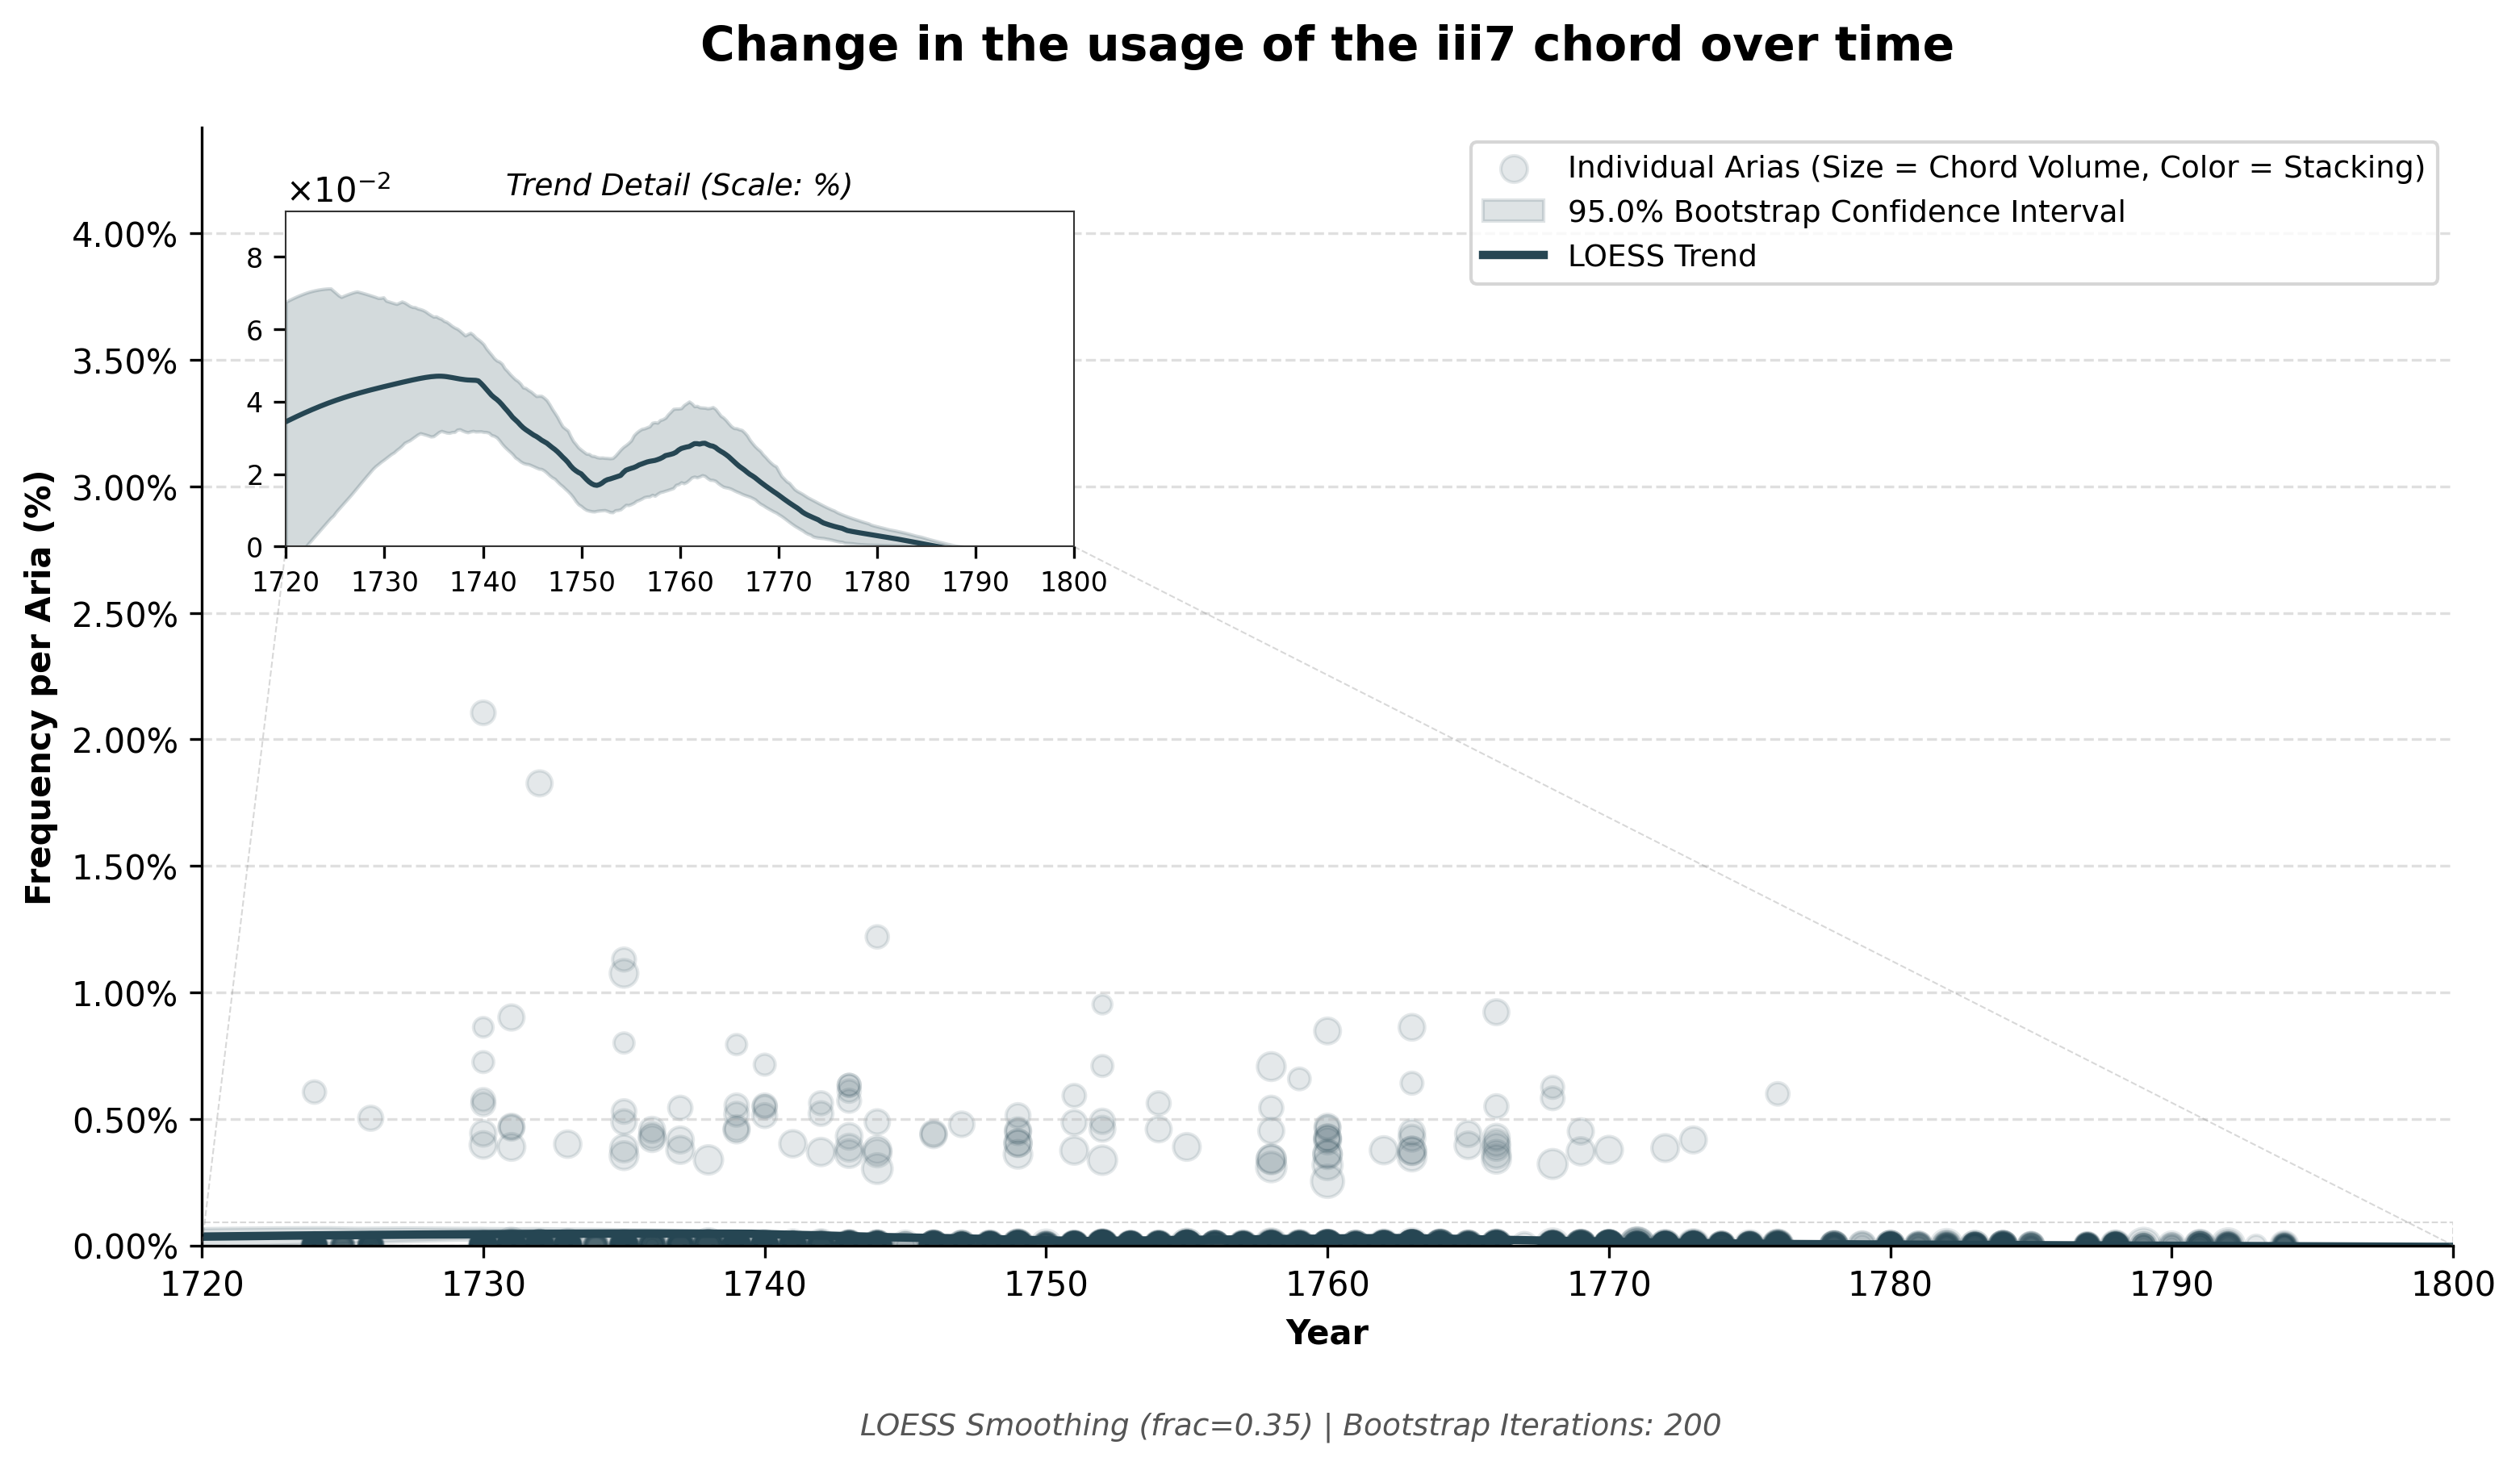
\includegraphics[width=\linewidth]{./images/chord_usage_timelines/loess_timeline_change_in_the_usage_of_the_iii7_chord_over_time.png}
    \caption{LOESS smoothed trend for the $\text{iii}^{7}$ chord frequency in the DIDONE corpus. The inset axis provides a magnified view of the trend line and bootstrap confidence interval, isolating the 0.0–0.06\% frequency range from the high-variance individual data points.}
    \label{fig:iii7_trend}
\end{figure}

A similar historical pattern was observed in the development of the Galant Style during the mid-eighteenth century: During this period, the frequency of predominant chords increased significantly as harmonic language moved beyond the dichotomy of tonic and dominant. With the emergence of the Classical style, this trend shifted back toward a consistent decline, eventually stabilizing at frequencies comparable to those of the middle Baroque. This evolution is again mirrored in the usage of individual chords, such as $\text{ii}^{6}$ and $\text{ii}^{6/5}$; their trajectory, which aligns with the broader development of predominant harmonies throughout the century, being illustrated in Figure \ref{fig:ii6_ii65_trend}.

\begin{figure}[htbp]
    \centering
    
\includegraphics[width=\linewidth]{./images/chord_usage_timelines/loess_timeline_change_in_the_usage_of_the_ii6_and_ii65_chords_over_time.png}
    \caption{LOESS smoothed trend for the $\text{ii}^{6}$ and $\text{ii}^{6/5}$ chord frequency in the DIDONE corpus.}
    \label{fig:ii6_ii65_trend}
\end{figure}

While many hypotheses regarding eighteenth-century musical development can be verified by observing individual chord frequency trends --- such as those shown in Figures \ref{fig:iii7_trend} and \ref{fig:ii6_ii65_trend} --- identifying correlations between these developments typically requires not only the base knowledge of the general trends to watch out for, but also laborious manual cross-referencing. Automated FPCA clustering alleviates this challenge by grouping chords with shared historical trajectories. Figure \ref{fig:fpca_clusters_6} demonstrates this approach, applied here to major-key arias to isolate stylistic shifts from fluctuations caused by changes in mode distribution.

\begin{figure*}[t]
    \centering
    
\includegraphics[width=\textwidth]{./images/fpca_clusters_major_keys_only.png }
    \caption{Clustering of chords that occur in at least 15\% of arias using FPCA and Loess smoothed trends.}
    \label{fig:fpca_clusters_6}
\end{figure*}

The resulting clusters align with established markers. Cluster 1 includes the $\text{ii}^{65}$ chord, while Cluster 4 captures specialized predominant and dominant-of-dominant harmonies, such as $\text{vii}^{\varnothing 7}\text{/V}$, both of which peaked during the Galant period. Cluster 3 contains chords characteristic of the Classical era, such as the $\text{V}^{(64)}$ suspension. In contrast, Cluster 2 groups chords that were prevalent during the Baroque but declined steadily toward the mid-eighteenth century, such as the first-inversion dominant and the minor tonic and its inversions. Finally, Cluster 6 tracks chords that maintained popularity longer, only declining toward the century's end --- notably the $\text{V}^{(4)}$ suspension, which was eventually superseded by the $\text{V}^{(64)}$ --- while Cluster 5 contains chronologically stable harmonies, such as the tonic $\text{I}$, that remained ubiquitous throughout the period. The exact clustered chords can be found in Table \ref{tab:chord_clusters}.

\begin{table}[htbp]
    \centering
    \small
    \renewcommand{\arraystretch}{1.3}
    \caption{Distribution of harmonic chords across identified clusters.}
    \begin{tabularx}{\columnwidth}{@{} l X @{}}
        \toprule
        \textbf{Cl.} & \textbf{Harmonic Chords} \\
        \midrule
        1 & ii$^{65}$, vii$^{\circ}$/V, vii$^{\varnothing 7}$, V$^{65}$/V, V$^{65}$/IV, I$^{(64)}$ \\ 
        \addlinespace[0.3em]
        2 & vii$^{\circ}$/IV, V$^6$, i, i$^6$, iv, VI, ii$^{\circ}$6, \#vii$^{\circ 6}$, iv$^6$, \#vii$^{\circ}$, iii, iii$^6$, vi$^6$, V/V \\ 
        \addlinespace[0.3em]
        3 & V$^{(64)}$, I$^{64}$, V$^{43}$, IV$^{64}$, ii$^2$, V$^7$, V$^7$/ii, I$^{(-1)}$, i$^{64}$, V$^2$/IV, V$^{7(+9)}$ \\ 
        \addlinespace[0.3em]
        4 & vii$^{\varnothing 7}$/V, I$^{(94)}$, vii$^{\circ 7}$/V, It$^6$ \\ 
        \addlinespace[0.3em]
        5 & I, V$^{65}$, V, IV, I$^6$, vii$^{\circ} 6$, vii$^{\circ}$, ii, V$^7$/IV, V$^{64}$, vi, vii$^{\circ 64}$, ii$^6$, V$^2$, vii$^{\circ 6}$/V, V$^{(6)}$ \\ 
        \addlinespace[0.3em]
        6 & IV$^6$, I$^{(4)}$, ii$^7$, ii$^{\varnothing 65}$, V$^7$/V, vi$^7$, \#vii$^{\circ 7}$, V$^{(4)}$ \\ 
        \bottomrule
    \end{tabularx}
    \label{tab:chord_clusters}
\end{table}



\section{Conclusion \& Future Work}\label{sec:conclusion}
The multi-tiered computational approach presented in this study provides a robust framework for visualizing and categorizing harmonic evolution in eighteenth-century opera. It demonstrates that combinations of different methods from data science can allow us to verify existing music theoretical assumptions and to establish a larger scale narrative of how musical language changed during the eighteenth century.

However, these findings also show the limitations of label-based modeling. While frequency trends capture the rise and fall of specific sonorities, they remain agnostic to the syntactical context in which these chords operate. Future work must therefore go beyond the analysis of individual notes and chords as uncontextualized data points and shift instead towards an integrated perspective that situates these harmonies within their surrounding micro- and macro-level structural frameworks.


% --- References ---
% example: \cite{finkensiepGENERALIZEDSKIPGRAMSPATTERN2018}.
\printbibliography

\end{document}